\newpage
\section{University}
%Since the address of the university corresponds to the address of who does the initial deploy, to login you need only to click on \emph{\textbf{Login}} at the top right of the screen.
%Once you've done this, 
After the login you will be redirected to the page represented in Figure~\ref{fig:loggedProfile}. As you can see, a black bar has appeared near the top of the screen.
The black bar contains on its left the voices \textbf{Academic Years}, \textbf{Degrees}, \textbf{Classes} and \textbf{Exams}. On the right it contains the voices \textbf{Administrators}, \textbf{Teachers} and \textbf{Students}.
The voices on the right allows the university to manage (create, visualize and delete) administrators, teachers and students.
\begin{figure}[!h]
\centering
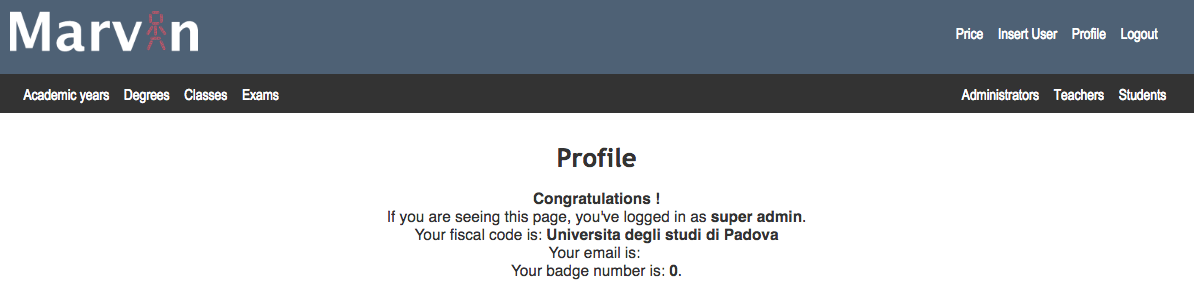
\includegraphics[width=1.0\textwidth]{img/loggedProfile.png}
\caption{Login with University}
\label{fig:loggedProfile}
\end{figure}

\subsection{Academic years}
By clicking on the \textbf{Academic years} voice in the black bar, you will see (as in Figure~\ref{fig:acadYear}) a register of all the academic years inserted in the system. For each academic year you can \emph{insert degrees} and \emph{delete the academic year}.
\begin{figure}[!h]
  \centering
  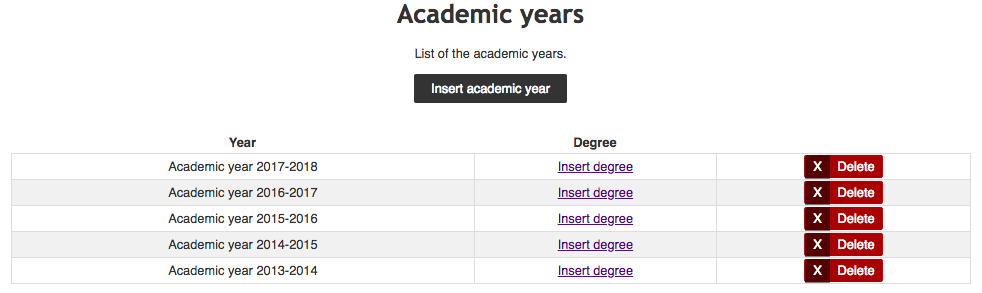
\includegraphics[width=1.0\textwidth]{img/accademicYears.png}
  \caption{Register of the the academic years in the system.}
  \label{fig:acadYear}
\end{figure}

\subsubsection{Creation of a new Academic Year}
Click on the button \textbf{Insert academic year}, you will be redirected to a page (like the one in Figure~\ref{fig:academicYInsertion}). Insert the name of the accademic year and click the \textbf{save} button. The name of the accademic year has to follow this simple rule: it must start with four digits followed by a ''\emph{-}'' character, which has to be	 followed by other four digits. The first digit of every block has to be ''2''. You cannot insert an accademic year that is older than the current year, for example, if we are in the year 2018, you cannot insert the accademic year 2017-2018.
\begin{figure}[!h]
	\centering
	
\includegraphics[width=0.80\textwidth]{img/academicYInsertion.png}
	\caption{Insertion of a new academic year in the system.}
	\label{fig:academicYInsertion}
\end{figure}

\subsubsection{Insertion of a degree} \label{sssec:degIns}
Click on \textbf{Insert degree}, you will be redirected to a page (like the one in Figure~\ref{fig:degreeInsertion}), insert a \emph{Degree description}  (for example ''Computer Science'') and, insert an unique code for that degree (for example ''CSLT17'), the code must be 6 characters long and it has to \emph{start with four capital letters} and \emph{end with two digits}. Click the \textbf{save} button.
\begin{figure}[!h]
  \centering
  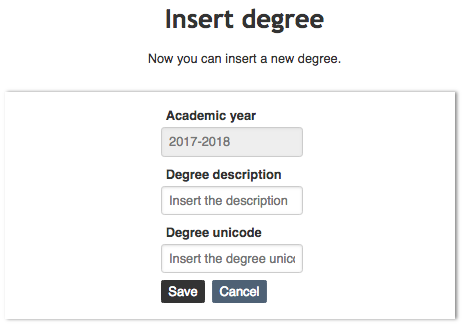
\includegraphics[width=0.55\textwidth]{img/degreeInsertion.png}
  \caption{Insertion of a degree.}
  \label{fig:degreeInsertion}
\end{figure}


\subsubsection{Deletion of an academic year}
Click on the \textbf{Delete} button, you will be redirected to a page (like the one in Figure~\ref{fig:deleteAcademicYear}), then click the \textbf{Delete} button to confirm the deletion.
\begin{figure}[H]
  \centering
  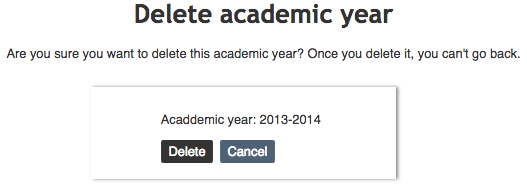
\includegraphics[width=0.80\textwidth]{img/deleteAcademicYear.png}
  \caption{Deletion of an academic year.}
  \label{fig:deleteAcademicYear}
\end{figure}

\subsection{Degrees}
By clicking on the \textbf{Degrees} voice in the menu, you will see (as in Figure~\ref{fig:chooseYear}) a page that asks you to choose an academic year. 
\begin{figure}[H]
	\centering
	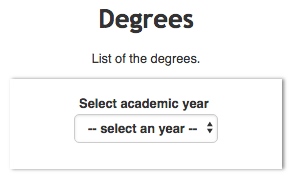
\includegraphics[width=0.35\textwidth]{img/chooseYear.png}
	\caption{Academic Years choice.}
	\label{fig:chooseYear}
\end{figure}

After choosing the academic year you want, the page will be updated with a list of all the degrees associated with that academic year (as in Figure~\ref{fig:degreeCourses}) . For each degree you can \emph{insert a class}  or \emph{delete the entire degree and all the classes associated with it}. If you want to insert a new degree, then click on the \textbf{Insert degree} button; the procedure is the same as the one described in~\ref{sssec:degIns}.
\begin{figure}[!h]
  \centering
  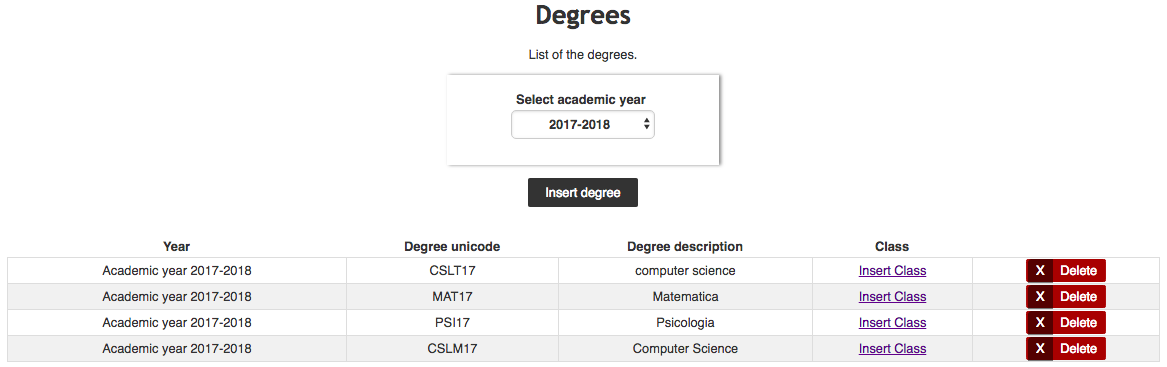
\includegraphics[width=1.0\textwidth]{img/degreeCourses.png}
  \caption{Register of the degrees related to a certain academic year in the system.}
  \label{fig:degreeCourses}
\end{figure}

\subsubsection{Insertion of a class} \label{sssec:clsIns}
To insert a class related to a degree, click on the link \textbf{Insert class} of the degree you choose. You will be redirected to a page like the one in Figure~\ref{fig:insertDidacticActivity}. Insert a class code (it must be formed by six characters, \emph{four capital letters} followed by \emph{two digits}, for example ''ALGO18'') and insert a brief description (for example ''Algorithms''). After that you will have to assign a teacher to the course. To do that, choose a teacher badge among those available in the list. A teacher badge can be available only if at least one teacher has been added to the system previously, to do that read \ref{subsec:exaIns}. After the badge number has been chosen, click the \textbf{Save} button.% and confirm the transaction by clicking on the MetaMask's \textbf{submit} button.
\begin{figure}[H]
  \centering
  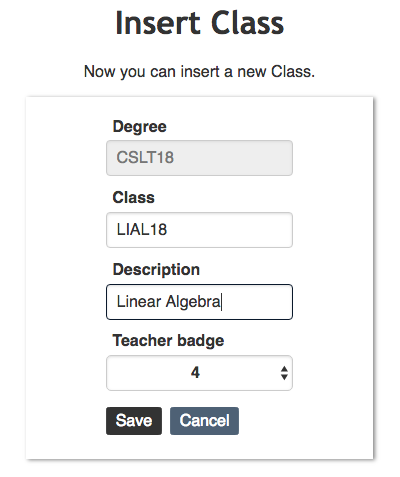
\includegraphics[width=0.30\textwidth]{img/insertDidacticActivity.png}
  \caption{Insertion of a class.}
  \label{fig:insertDidacticActivity}
\end{figure}

\subsubsection{Deletion of a degree}
To delete a degree, click on \textbf{Delete} button of the degree you choose. You will be redirected to a page (like the one in Figure~\ref{fig:deleteDegree}). Click the \textbf{Delete} button and confirm.% the transaction by clicking on the MetaMask's \textbf{submit} button.
\begin{figure}[H]
  \centering
  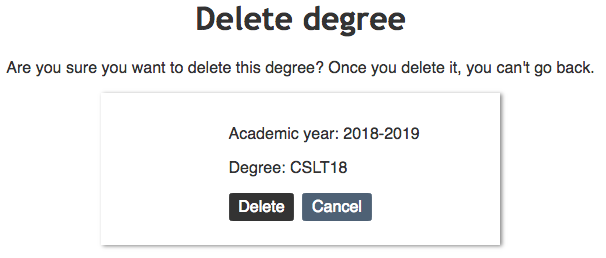
\includegraphics[width=0.65\textwidth]{img/deleteDegree.png}
  \caption{Deletion of a degree.}
  \label{fig:deleteDegree}
\end{figure}

\subsection{Classes}
By clicking on the \textbf{Classes} voice in the menu, you will see (as in Figure~\ref{fig:chooseClass}) a page that asks you to choose an academic year and then one of its degree programs.
\begin{figure}[!h]
	\centering
	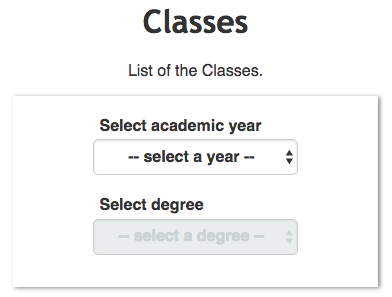
\includegraphics[width=0.35\textwidth]{img/chooseClass.png}
	\caption{Choice of an academic year and one of its degree programs .}
	\label{fig:chooseClass}
\end{figure}

After choosing the academic year and the degree program you want, the page will be updated with a list of all the classes (as in Figure~\ref{fig:classes}) . For each class you can \emph{insert an exam}  or \emph{delete the class}. If you want to insert a new class, then click on the \textbf{Insert Class} button; the procedure is the same as the one described in~\ref{sssec:clsIns}
\begin{figure}[!h]
	\centering
	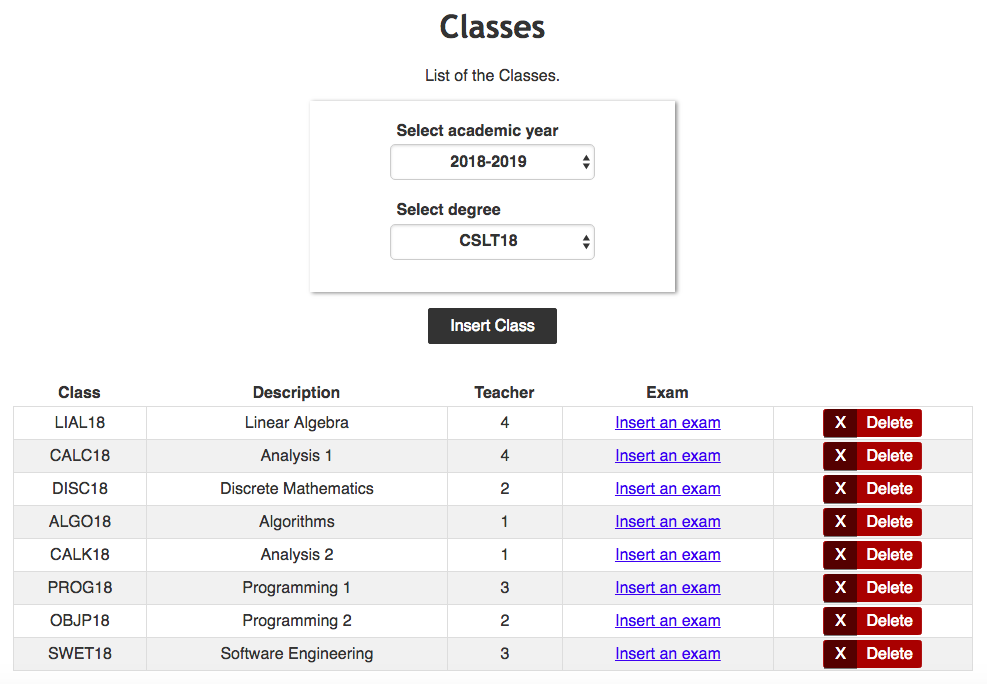
\includegraphics[width=1.0\textwidth]{img/classes.png}
	\caption{Register of the classes of the Computer Science degree.}
	\label{fig:classes}
\end{figure}

\subsubsection{Insertion of an exam} \label{subsec:exaIns}
To insert an exam related to a class, click on the link \textbf{Insert exam} of the class you choose. You will be redirected to a page like the one in Figure~\ref{fig:insertExam}. Choose the type of the exam (\emph{written, oral, practice}), write the name of the place in which the exam will be helded, insert the date and the time and a Unicode. A valid Unicode consists of the class code followed by ''-'' followed by two digits between ''00'' and ''99''. The date of the exam must be later than the current day and the time must be inserted in a range between ''8:30'' and ''17:30''
\begin{figure}[H]
	\centering
	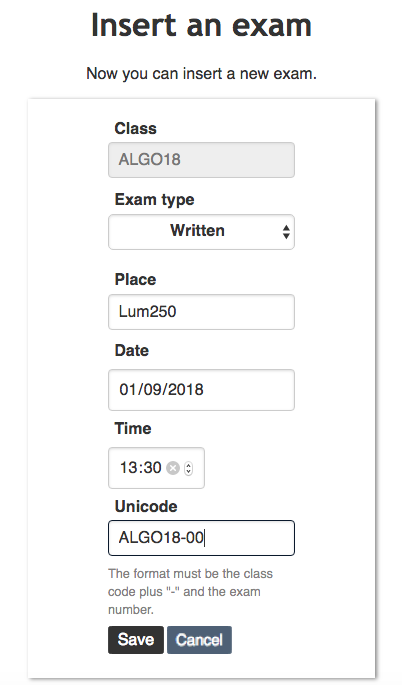
\includegraphics[width=0.35\textwidth]{img/insertExam.png}
	\caption{Insertion of an exam in the system.}
	\label{fig:insertExam}
\end{figure}

\subsubsection{Deletion of a class}
To delete a class click on its \textbf{Delete} button. You will be redirected to a page (like the one in Figure~\ref{fig:deleteClass}). Click the \textbf{Delete} button.% and confirm the transaction by clicking on the MetaMask's \textbf{submit} button.
\begin{figure}[H]
	\centering
	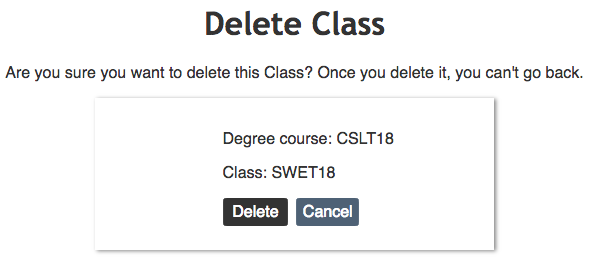
\includegraphics[width=0.65\textwidth]{img/deleteClass.png}
	\caption{Deletion of a class.}
	\label{fig:deleteClass}
\end{figure}

\subsection{Administrators, Teachers and Students management} \label{subsec:ats}
When you choose a voice on the right side of the black bar located near the top of the screen, you're selecting a category between \emph{Administrators}, \emph{Teachers} and \emph{Students}.  Depending on your choice, you will see a list of administrators, or teachers or students, for example a list like the one in Figure~\ref{fig:userList}. As you may notice looking at the table in the figure, the cell of the column named ''\emph{Is signed up}'' has a green dot if the inserted user has logged in, otherwise it has a red dot. An inserted user that never signed up can be eliminated by clicking on the relative deleted button.
\begin{figure}[H]
	\centering
	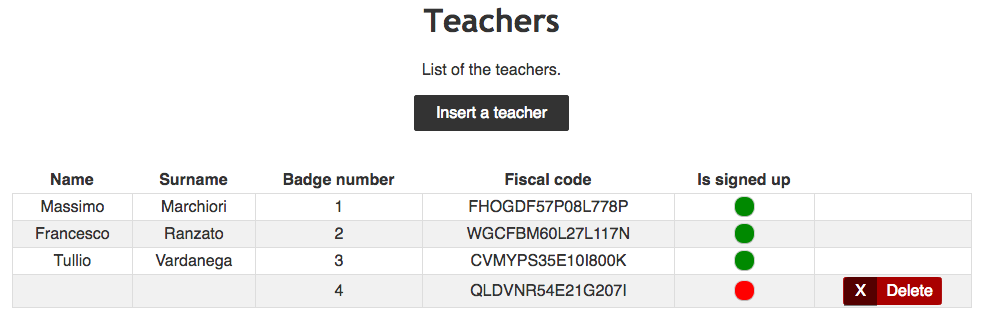
\includegraphics[width=1.0\textwidth]{img/userList.png}
	\caption{List of the teachers in the system.}
	\label{fig:userList}
\end{figure}

\subsubsection{User Insertion}
Inserting an user in the system is an operation that has two phases: 
\begin{itemize}
	\item The first one requires that the university (or an admin) clicks on the correct voice (he/she has to choose between \emph{administrators, teachers, students}) in the black bar depending on the type of user he/she want to insert and then, clicks on the button \textbf{Insert an admin} (respectively \textbf{Insert a teacher}, \textbf{Insert a student}) to creates a new account in the system.
	
	You will be redirected to a page similar to the one in Figure~\ref{fig:userInsertionStudent}. Then you'll have to inserting the fiscal code of the user and an unique code of ten digits. If the user is a Student, then you have to select also an academic year and a degree.
	
	You can also insert an user by clicking the \textbf{Insert user} button in the blue bar located on the top of every page;
	\begin{figure}[H]
		\centering
		%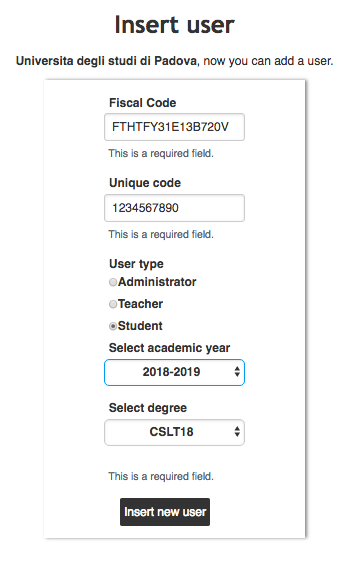
\includegraphics[width=0.65\textwidth, height=3in]{img/userInsertionStudent.png}
		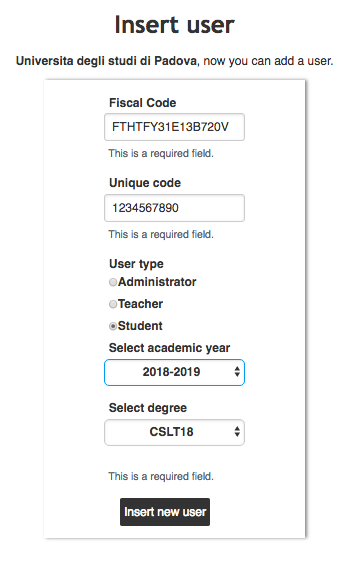
\includegraphics[width=0.35\textwidth]{img/userInsertionStudent.png}
		\caption{Student insertion by an admin or university account}
		\label{fig:userInsertionStudent}
	\end{figure}
	
	\item The second one is necessary to authenticate and identify the new user: in fact, the  new user during the Sign Up will have to insert its own Fiscal Code and the Identification Code issued by the university (or an admin), and other data as in Figure~\ref{fig:stdSignUp}. If this two data (Fiscal Code and Identification Code) are the same as those inserted by the University (or an admin), then all the user's personal data will be saved and its Metamask address connected to the account, so that the next logins can be made automatically.
	If the form has been filled correctly, then a Metamask window will be opened in front of you. Confirm clicking the \textbf{SUBMIT} button.
	\begin{figure}[H]
		\centering
		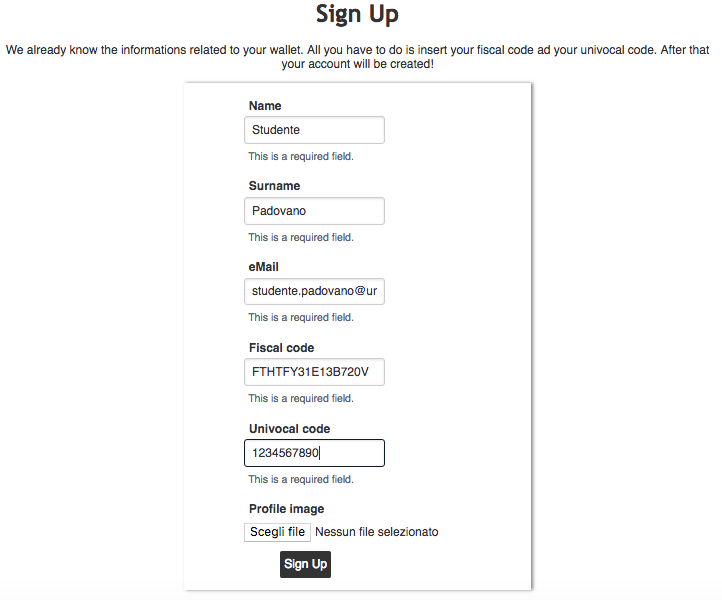
\includegraphics[width=0.65\textwidth]{img/stdSignUp.png}
		\caption{User Sign Up}
		\label{fig:stdSignUp}
	\end{figure}
\end{itemize}

\newpage
\section{Administrators}
An administrator has the same privileges of the university user but he/she can't create new administrator users.






